\section{Results}
\subsection{Simulation Results}
%_______________________________________________________________________%
\begin{frame}{Implementation on Matlab}
    \begin{figure}
        \centering
        \includegraphics[width=0.9\linewidth]{imgs/Simulation/MFC_efficient_model.pdf}
        \caption{Simulink Model MFC Loop}
        \label{fig:Simulink Model MFC Loop}
    \end{figure}
\end{frame}


%_______________________________________________________________________%
\begin{frame}{Set‐Point Tracking in the Experiment}
    Here is the desired trajectory : 
    \begin{figure}
        \centering
        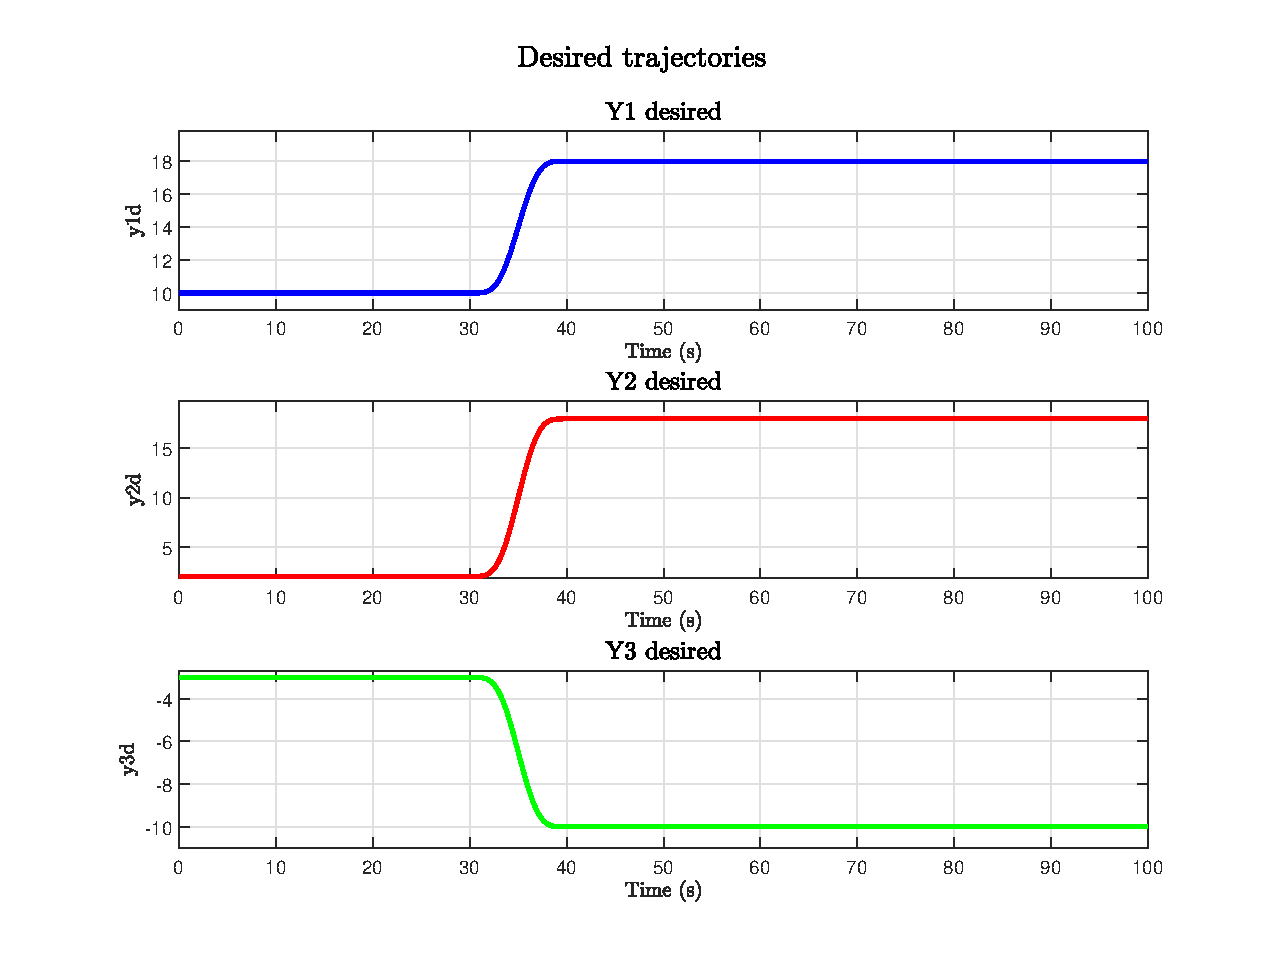
\includegraphics[width=0.75\linewidth]{imgs/Simulation/desiredTraj.eps}
        \caption{Desired Trajectories of the Load}
    \end{figure}
\end{frame}


\begin{frame}{Simulation Results}
\begin{figure}
    \centering
    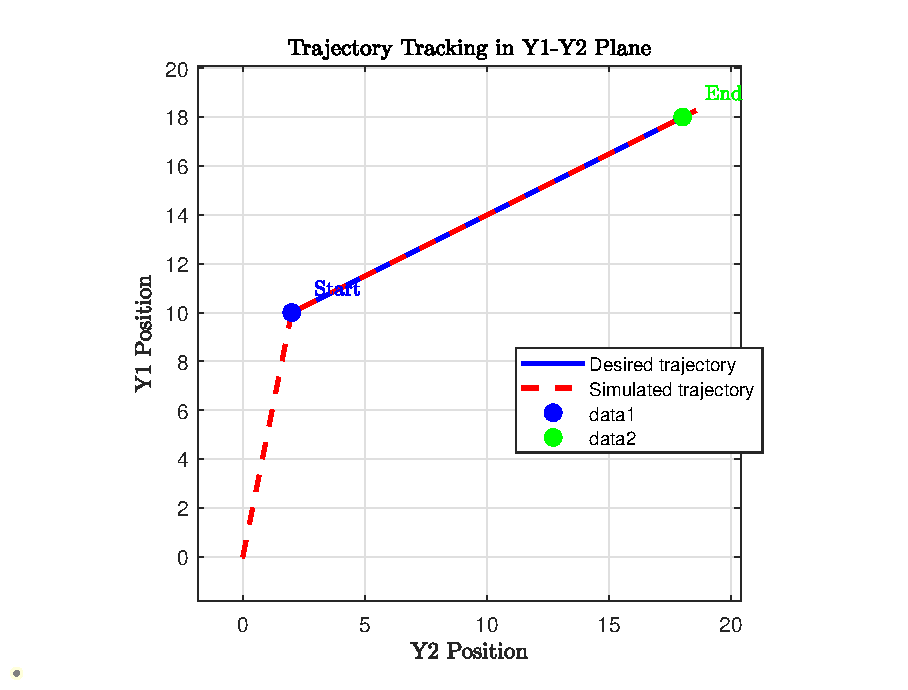
\includegraphics[width=0.8\linewidth]{imgs/Simulation/XYTrajectory.eps}
    \caption{Difference between CI desired states and Model States}
\end{figure}

\end{frame}



\begin{frame}{Simulation Results}
\framesubtitle{High Gain}
    \begin{figure}
    \centering
    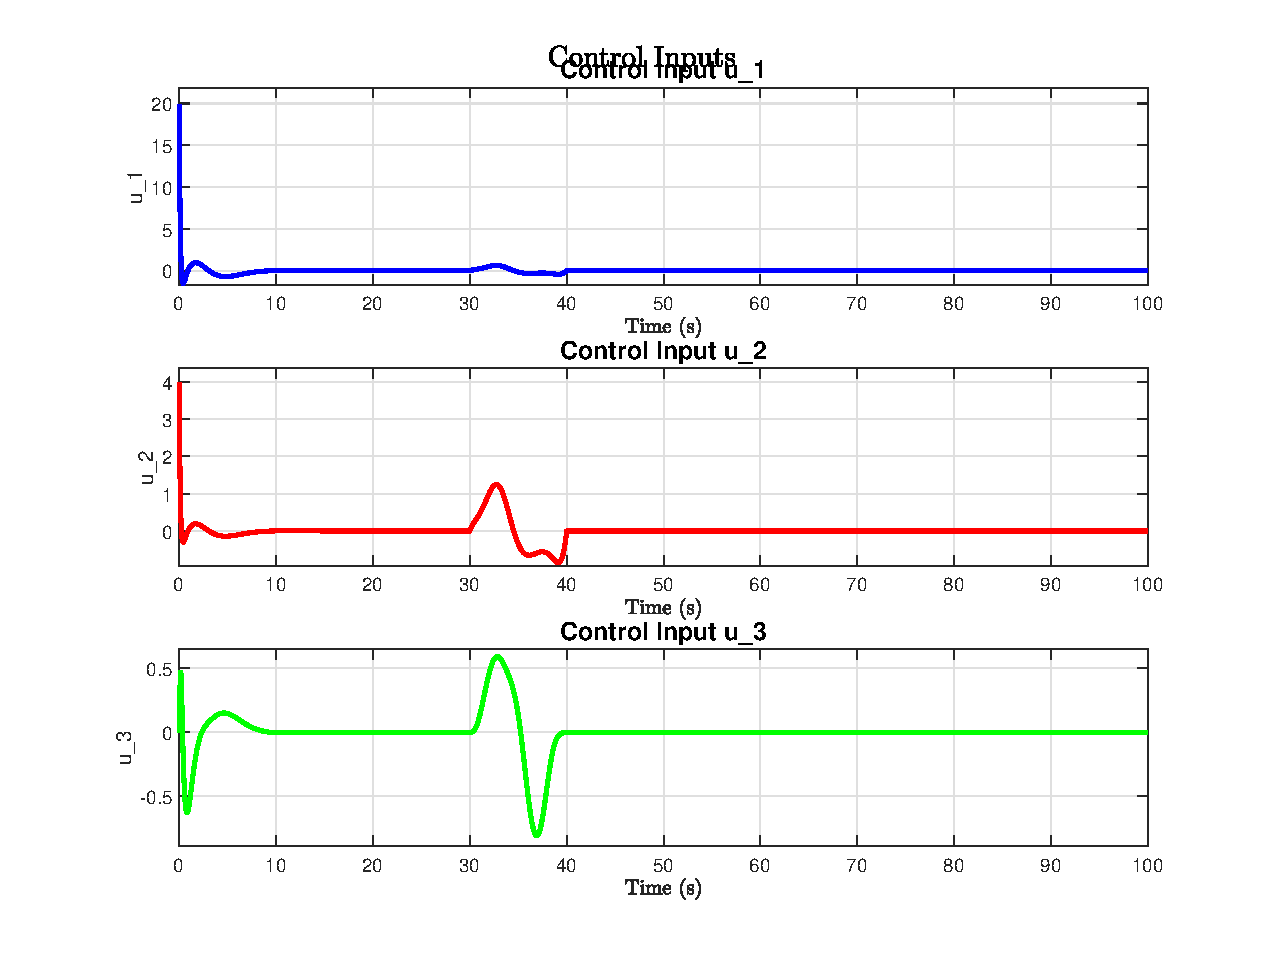
\includegraphics[width=0.8\linewidth]{imgs/Simulation/u_HG.eps}
    \caption{Input for Set point tracking High gain control}
\end{figure}
\end{frame}


\begin{frame}{Simulation Results}
\framesubtitle{MFC}
    \begin{figure}
        \centering
        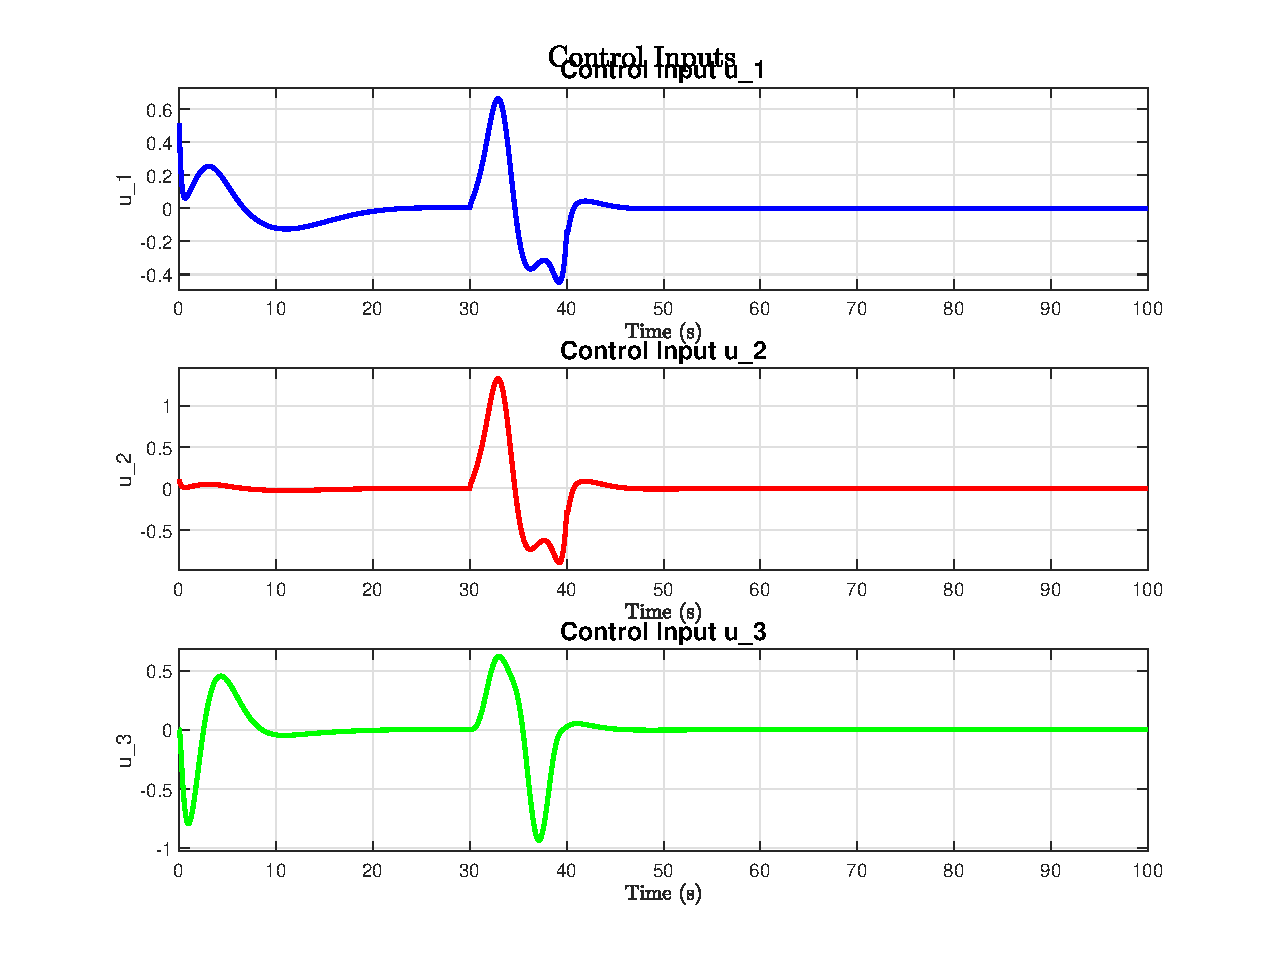
\includegraphics[width=0.8\linewidth]{imgs/Simulation/u_efficientMFC_Good_CI.eps}
        \caption{Input for Set point tracking MFC}
        \label{fig:input-mfc}
    \end{figure}
\end{frame}




    







%_______________________________________________________________________%
\subsection{Real Plant Experiment}
\begin{frame}{Presentation}
\framesubtitle{The Trolley and the Load}

\begin{figure}
    \centering
    \rotatebox{270}{\includegraphics[width=0.5\linewidth]{imgs/Simulation/Trolley.jpg}}
    \caption{Zoom on the crane's trolley}
\end{figure}
\end{frame} 

\begin{frame}{X and Y motors}
\begin{columns}[T] % [T] aligns the columns at the top
    \begin{column}{0.5\textwidth} % Specify width for the first column
        \centering
        \rotatebox{270}{\includegraphics[width=\linewidth]{imgs/Simulation/Xmot.jpg}}
        \captionof{figure}{Zoom on X motor}
    \end{column}
    \begin{column}{0.5\textwidth} % Specify width for the second column
        \centering
        \rotatebox{270}{\includegraphics[width=\linewidth]{imgs/Simulation/Ymot.jpg}}
        \captionof{figure}{Zoom on Y motor}
    \end{column}
\end{columns}
\end{frame}

%_______________________________________________________________________%
\begin{frame}{Results}   
\end{frame}